\documentclass[]{article}

\usepackage[spanish]{babel}

%para agregar párrafos predifinidos
\usepackage{lipsum}
\usepackage{amsmath,amssymb}
\usepackage{graphicx}
\usepackage{xcolor}

%agreguemos el paquete array
\usepackage{array}   %F5 para compilar, F7 para visualizar


\title{CDE \LaTeX }
\author{clase 5}
\date{27 de marco del 2023}

\begin{document}   %todo entorno es con begin
	\maketitle
	\begin{abstract}
	\lipsum[3-4]
	\end{abstract}

\section{el entorno tabular}
\noindent{Sintaxis}
\begin{verbatim}
\begin{tabular}[posicion]{Definicion}
	a_{11} & a_{12} & a_{13}  \\
	a_{21} & a_{22} & a_{23}
	\end{tabular}
\end{verbatim}

Profundicemos en el argumento \verb*|Definicion| :
Definiremos el número de columnas y la justificación de cada uan de esas columnas.

\begin{itemize}
	\item Usar las letras \verb*|l| (left), \verb*|c| (center) y \verb*|r| (right) para justificar el texto dentro de una columna
\begin{verbatim}
	\begin{tabular}[]{lrrc}
		a_{11} & a_{12} & a_{13}  & a_{14} \\
		a_{21} & a_{22} & a_{23}& a_{24}
	\end{tabular}
\end{verbatim}	

Veamos un ejemplo
	\begin{tabular}[]{lrrc}
	$a_{11}$ & $a_{12}$ & $a_{13}$  & $a_{14}$ \\
	$a_{21}$ & $a_{22}$ & $a_{23}$& $a_{24}$
\end{tabular}


	Veamos otro ejemplo
	\begin{tabular}[]{lrrc}
		$a_{11}$ & $a_{12}$ & $a_{13}$  & $a_{14}$ \\
		$a_{21}$ & $a_{22}$ & $a_{23}$& \lipsum[2]
	\end{tabular}
\item Definamos un párrafo como elemento de un \verb*|tabular|

VEamos un ejemplo:


	\begin{tabular}[]{lrrp{9cm}}   %asi 3,6,9 cmse puede aumenta el ancho
	$a_{11}$ & $a_{12}$ & $a_{13}$  & $a_{14}$ \\
	$a_{21}$ & $a_{22}$ & $a_{23}$& \lipsum[2]
\end{tabular}

Nota el uso de lineas horizontales con \verb*|hline|


En ejecución
\begin{center}
	\begin{tabular}[]{|c|c|c|}
	\hline 
		$a_{11}$ & $a_{12}$ & $a_{13}$  \\
	\hline	
		$a_{21}$ & $a_{22}$ & $a_{23}$  \\
	\hline
	\end{tabular}
\end{center}



\subsection {cline}
El comando \verb*|cline{i-j}| trazará a línea horizontal entre las columnad de la \verb*|i| a la  \verb*|j|
\begin{center}
	\begin{tabular}[]{cccr}
		\hline 
		Producto & Precio unitario &cantidad &subtotal \\
		\hline	
		MOnitores & 1250 & 2 & 2500 \\
		          & 2780 & 2 & 5560 \\
		          & 16800 & 4 & 67200 \\
		 \hline
		 GPU      & 2500 & 2 & 5000 \\
		          & 3700 & 3 & 11100 \\
		          \cline{4-4}   %esta permite subyrayar solo una parte
		          &      &   & 78300
		
	\end{tabular}

\end{center}

	\end{itemize}




\subsection {Encolumnar el punto decimal}
Consideremos que tenemos 4 números punto flotante , donde cada uno de estos números posee una distinta cantidad de cifras en la mantisa: 3.14159, 2.71, 123.4567 y 0.
\begin{center}
	\begin{tabular}[]{cc}
		\hline 
		Var1 & 3.14159 \\
		Var2 & 2.71 \\
		Var3 & 123.4567 \\
		Var4 & 0 \\
		\hline	
			
		\end{tabular}
	\end{center}


	
Consideremos arreglar y encolumnar de las ubicación del punto decimal
\begin{center}
	\begin{tabular}[]{cr@{.}l}
		Varios &  cifras & \\
		\hline 
		Var1 & 3&14159 \\
		Var2 & 2&71 \\
		Var3 & 123&4567 \\
		Var4 & 0 &\\
		\hline	
		
	\end{tabular}
\end{center}	
	
\section{Construcción de figuras}	
\lipsum[2-5]
\begin{figure}[h]
	\centering
	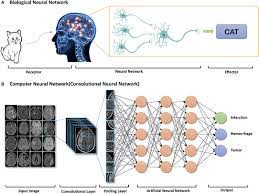
\includegraphics[width=0.6\textwidth]{Figure/deepray.jpg}
	\caption{deep learning para rayos}
	\label{fig: deep}
	\end{figure}

\begin{figure}[h]
	\centering
	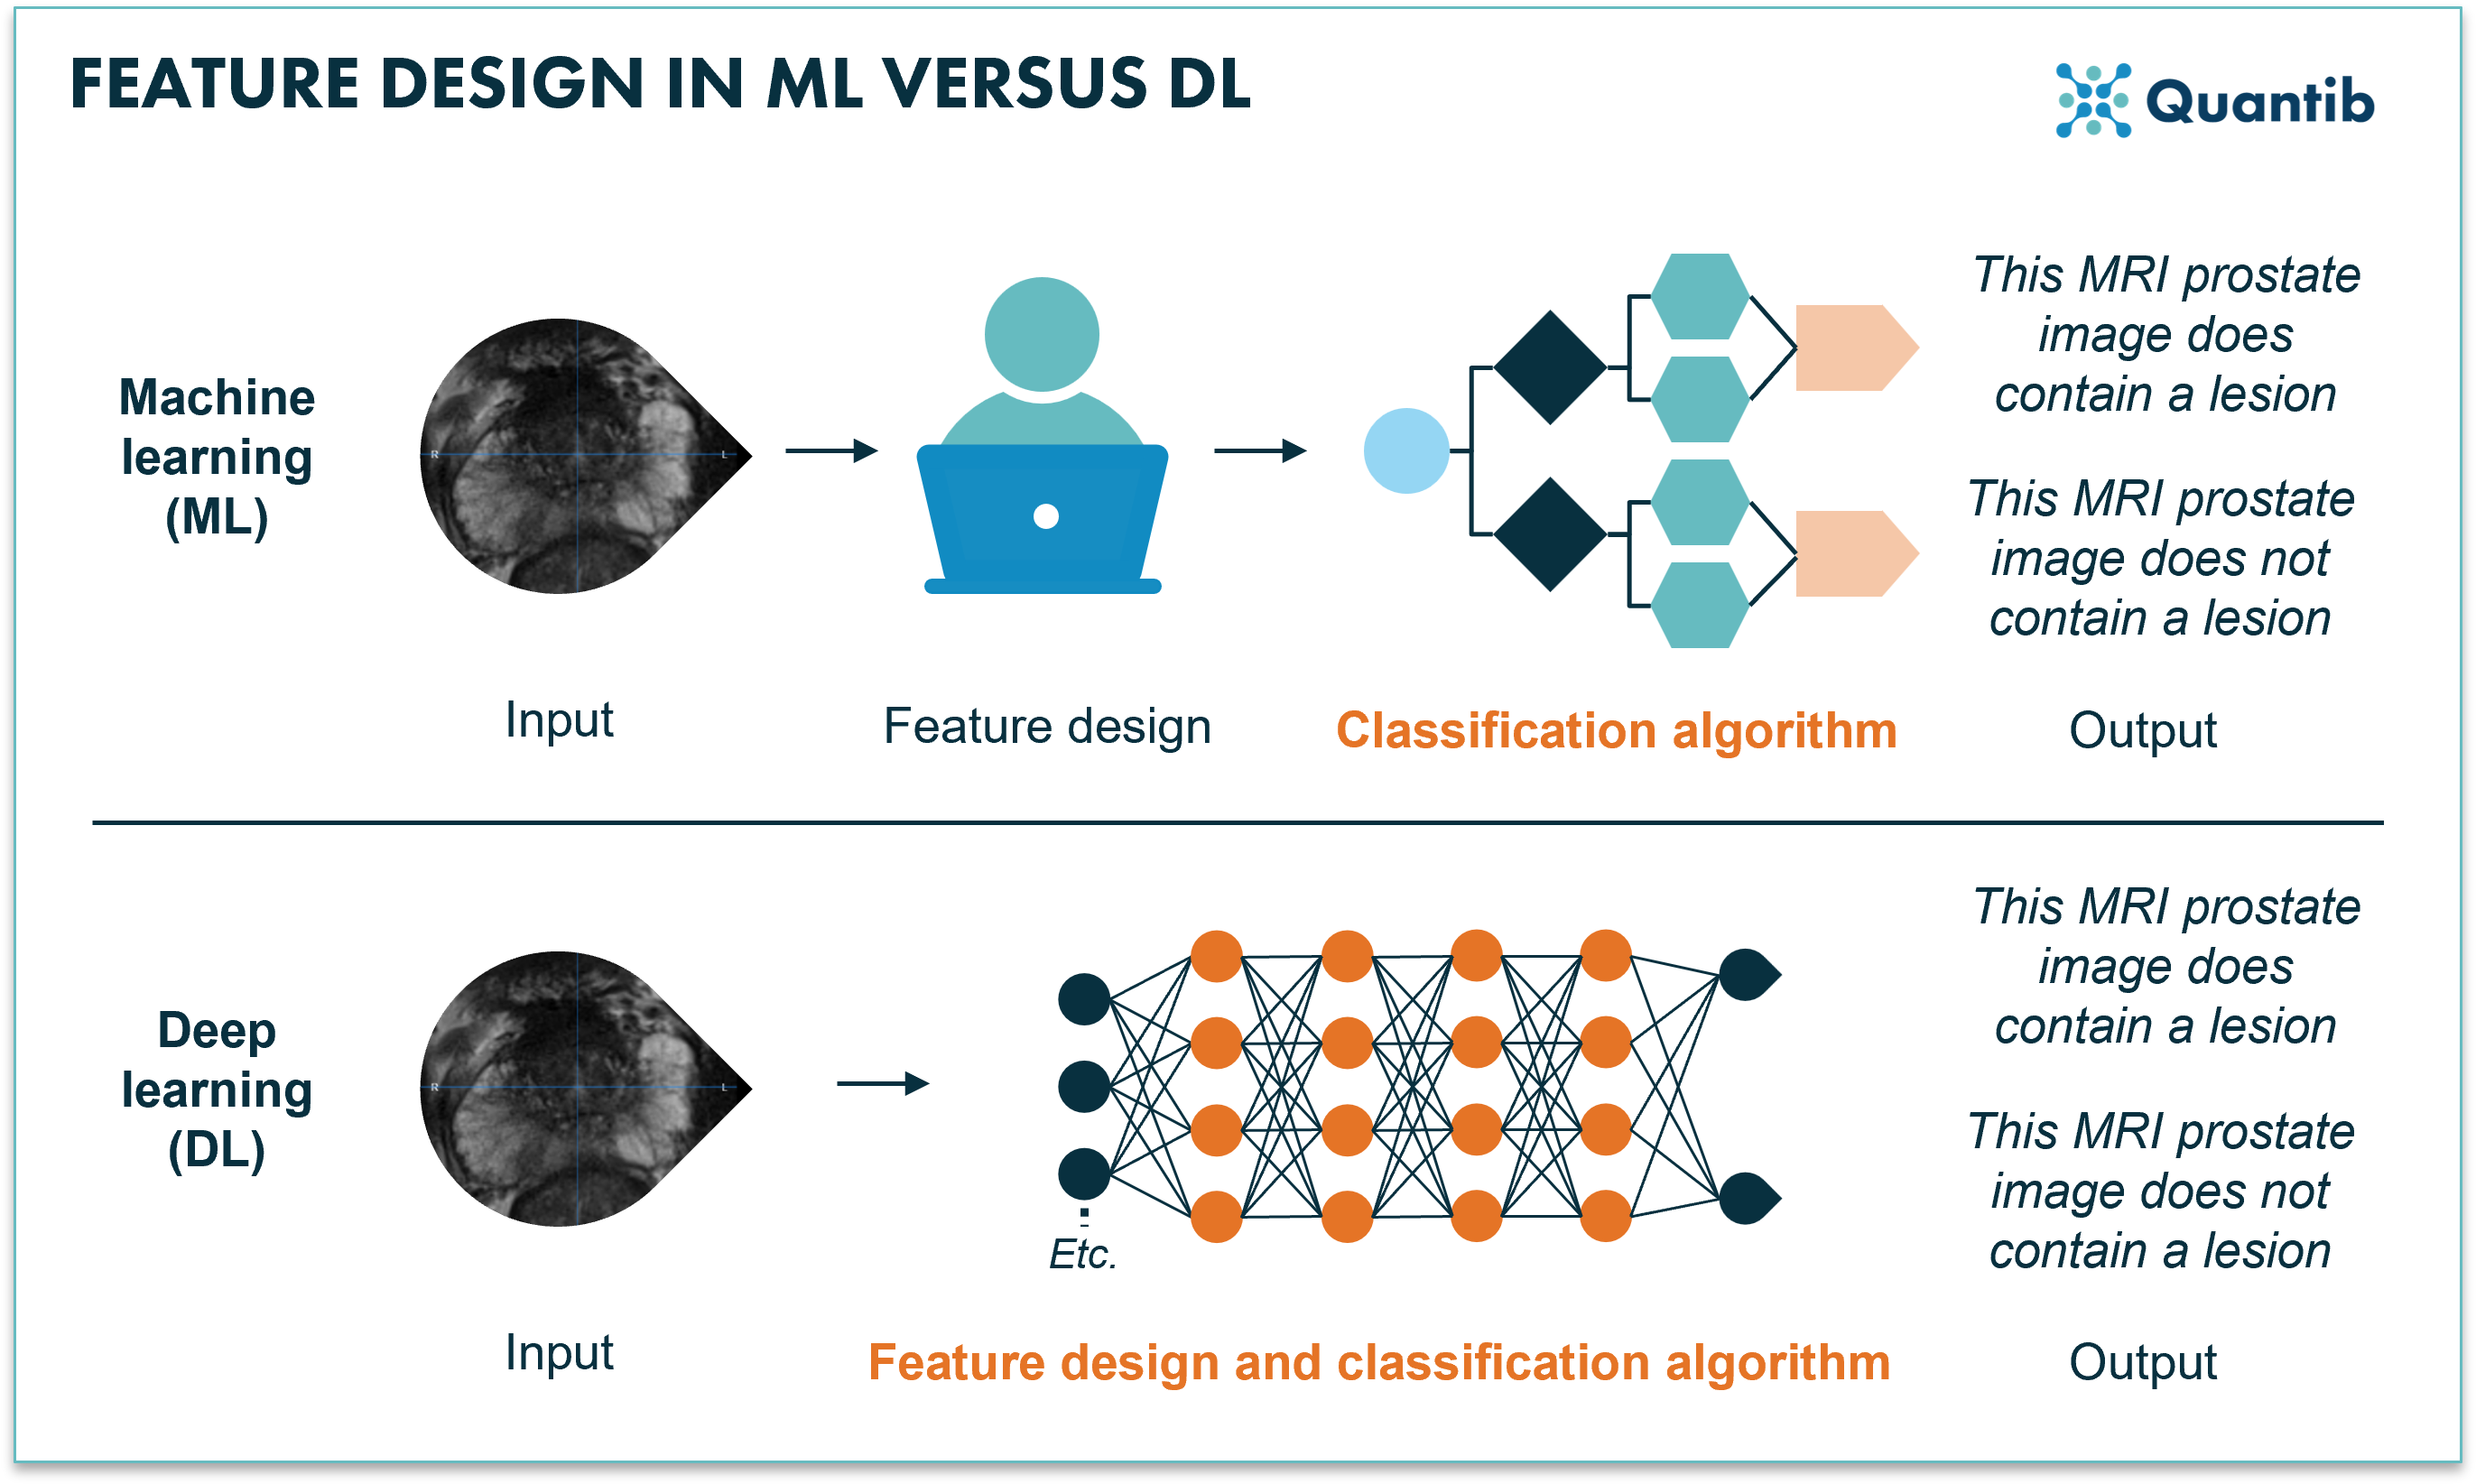
\includegraphics[width=0.6\textwidth]{Figure/redesray}
	\caption{redes}
	\label{fig: rede}
\end{figure}
\lipsum[2-5]

\begin{figure}[h]
	\centering
	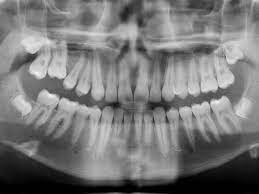
\includegraphics[width=0.6\textwidth]{Figure/primera}
	\caption{text}
	\label{key}
\end{figure}




%para atblas es table
	
\section{Construcción del índice de tablas}	
\lipsum[12-14]
\begin{table}[h]
	\centering
	\begin{center}
		\begin{tabular}[]{cr@{.}l}
			Varios &  cifras & \\
			\hline 
			Var1 & 3&14159 \\
			Var2 & 2&71 \\
			Var3 & 123&4567 \\
			Var4 & 0 &\\
			\hline	
			
		\end{tabular}
	\end{center}	
\caption{Costos}
\label{table:1}

\end{table}
	

	FIN.
	
\newpage	
	\listoftables
	\listoffigures
	\tableofcontents
	
\end{document}